\chapter{Numbers and Reality}
\label{chap:II_numbers}

% =====================================================
% 2.1 Natural Numbers and Counting
% =====================================================
\subsection{Natural Numbers and Counting}
\label{sec:2.1_natural_numbers}

The history of \emph{numbers}\index{numbers} begins with the human need
to order the surrounding world.
Long before there was \emph{writing}\index{writing} or
developed \emph{calculation methods}\index{calculation methods},
people used \emph{counting}\index{counting} to keep track of animals,
tools, supplies, or days.
Counting was a fundamental \emph{cultural technique}\index{cultural technique}
without which \emph{trade}\index{trade},
\emph{planning}\index{planning}, and
\emph{science}\index{science}
would hardly have been conceivable.

Yet even here something fundamental becomes visible:
human beings invent signs, words, and methods of calculation,
but they do so in response to something real.
Where quantities are distinguished, compared, and ordered,
a structure emerges that is not arbitrary.
Precisely there lies the origin of the natural numbers.

\subsubsection*{Earliest Beginnings}
\phantomsection
Archaeological finds\index{archaeology} suggest that already
around 20,000 to 35,000 years ago, \emph{counting aids}\index{counting aids}
were being used.
Particularly well known is the \emph{Ishango bone}\index{Ishango bone},
which was discovered in Central Africa in 1960 by
Jean de Heinzelin de Braucourt\index{Heinzelin de Braucourt, Jean de}.
Even older is the \emph{Lebombo bone}\index{Lebombo bone}
from South Africa.
Both artifacts suggest that people in the
\emph{Paleolithic period}\index{Paleolithic period}
recorded quantities by means of notches (see Fig.~\ref{fig:bones}).

\newpage
\noindent
\begin{figure}[ht]
	\centering
	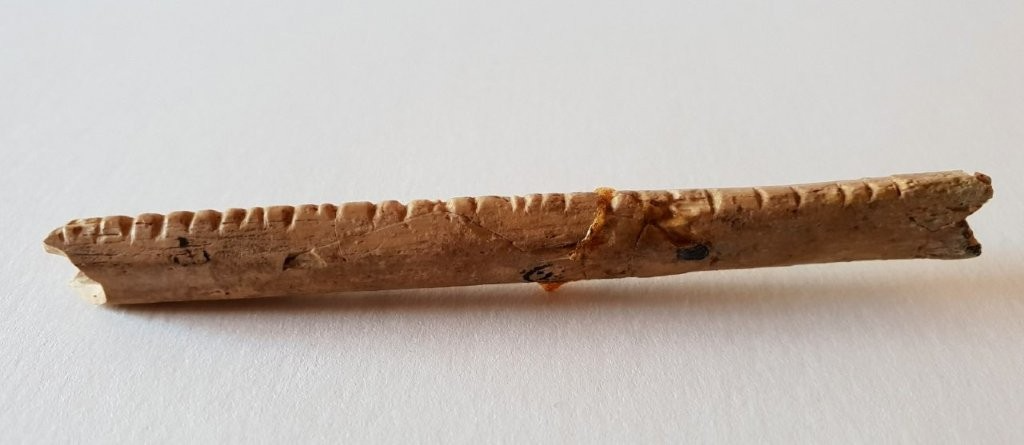
\includegraphics[width=0.45\textwidth]{bilder/lebombo-bone.png}
	\hfill
	\includegraphics[width=0.45\textwidth]{bilder/ishango_bone.jpg}
	\caption{Left: Lebombo bone (about 35,000 years old, South Africa).
		Right: Ishango bone (about 20,000 years old, Central Africa).
		Both show regular notches that are interpreted as early counting aids.
		The Ishango bone is now kept at the \emph{Royal Belgian Institute of Natural Sciences} in Brussels.}
	\label{fig:bones}
\end{figure}

\begin{HistoryBox}[The Ishango Bone]
	The \emph{Ishango bone} was discovered in Central Africa in 1960 by
	Jean de Heinzelin de Braucourt and is about 20,000 years old.
	
	The bone contains three columns of notches
	that are not randomly distributed, but appear to be arranged in groups.
	It probably served as a kind of \emph{tally stick}\index{tally stick} --
	possibly for observing the \emph{lunar cycle}\index{lunar cycle}
	or for counting supplies.
	
	It is especially striking that some groupings have been associated with
	\emph{prime numbers}\index{prime numbers}
	(11, 13, 17, 19).
	Whether this was intentional or accidental remains open.
	What is certain, however, is this:
	the bone shows that already in the Paleolithic period,
	humans recognized regular patterns and not only perceived quantities,
	but deliberately recorded them.
	\label{box:ishango}
\end{HistoryBox}

In other places as well, people used notches, knots, or stones as simple counting aids.
Tally sticks served for thousands of years to record supplies, dues, or debts --
well into the modern period, for example in Alpine regions.
What is remarkable here is less the external form than the underlying idea:
independently of one another, different cultures adopted similar means
to make quantities visible and comparable.

\subsubsection*{From Counting to the Concept of Number}
\phantomsection
In addition to archaeological finds, \emph{linguistics}\index{linguistics}
also shows that humans initially divided their environment only roughly
into small and large quantities --
roughly according to the pattern ``one,'' ``two,'' and ``many.''

Some traditional cultures still have only very few
\emph{number words}\index{number words},
often merely simple distinctions of this kind,
for example in parts of \emph{Papua New Guinea}\index{Papua New Guinea}
or \emph{Australia}\index{Australia}.

This shows:
number words, number symbols, and methods of calculation are not self-evident.
They are cultural achievements.
They arise from practical needs such as
\emph{trade}\index{trade},
\emph{keeping supplies}\index{keeping supplies},
or \emph{calendar calculation}\index{calendar calculation}.

But what these forms refer to is not arbitrary.
Where humans count, compare, and order,
they encounter real differences between quantities.
Everywhere -- in Africa, Asia, Europe, or Oceania --
people therefore developed counting aids and
\emph{concepts of number}\index{concept of number},
because reality itself contains structures
that can be expressed in numbers.

The natural numbers thus appear not as a mere invention,
but as a first linguistic and symbolic formulation
of an order that is already present in the world.

\newpage
\noindent

% =====================================================
% 2.2 Irrational Numbers -- the Crisis of the Greeks
% =====================================================
\subsection{Irrational Numbers -- the Crisis of the Greeks}
\label{sec:2.2_irrational}

\subsubsection*{Starting Point: Pythagoras and the Pythagoreans}
\phantomsection
The early Greek mathematicians\index{Greeks},
especially the school of the \emph{Pythagoreans}\index{Pythagoreans},
were convinced that the world could be described completely
by \emph{whole numbers}\index{whole numbers} and \emph{fractions}\index{fractions}.
Their guiding principle was: ``All is number.''
What this meant above all was:
everything can be expressed by ratios of whole numbers.
The \emph{Pythagorean theorem}\index{Pythagorean theorem}
was a central symbol of this conviction.

\subsubsection*{First Insight: No Common Measure (Incommensurability)}
\phantomsection
Yet precisely this theorem led to a result
that no longer fit the previous worldview.
If one considers a square with side length $1$,
then the length of the diagonal is given by
\[
c^2 = 1^2 + 1^2 = 2
\quad \Rightarrow \quad
c = \sqrt{2}.
\]

But exactly here a problem appeared:
the number $\sqrt{2}$ cannot be represented as a fraction of two whole numbers.
Thus it became clear:
there are \emph{incommensurable lengths}\index{incommensurability},
that is, lengths that have no common measure.
The side length $1$ and the diagonal $\sqrt{2}$ are incommensurable.

This insight shook the basic conviction of the Pythagoreans.
For if even such a simple geometric object as a square
produces a length that cannot be written as a fraction,
then the world is apparently not completely describable
by whole numbers and their ratios.

\subsubsection*{The Crisis of the Greeks}
\phantomsection
The discovery of irrationality therefore meant more
than a technical difficulty.
It struck at the core of Pythagorean thinking.
According to tradition, \emph{Hippasus of Metapontum}\index{Hippasus of Metapontum}
is said to have recognized this fact.
A later legend even reports
that he was drowned by his companions
because he had revealed this ``secret.''
Whether this story is historically accurate is uncertain.
What is certain, however, is this:
the discovery of irrational quantities confronted Greek mathematics
with a fundamental problem
and led to deeper reflection on number, measure, and proof.

\newpage
\noindent
\subsubsection*{The Proof}
\phantomsection
A rigorous proof of the irrationality was formulated by \emph{Euclid}\index{Euclid}
in Book X of his \emph{Elements}\index{Elements (Euclid)}.
It is based on a classic proof by contradiction:

\begin{MathBox}[Proof by Contradiction for $\sqrt{2}$]
	\phantomsection	\label{box:contradiction}
	Assume that $\sqrt{2}$ is rational, so that $\sqrt{2}=\tfrac{p}{q}$ with
	whole numbers $p,q$ that have no common divisor.
	Then $2q^2=p^2$.
	It follows that:
	$p^2$ is even, and therefore $p$ is even.
	If we write $p=2r$, then
	$2q^2=(2r)^2=4r^2$, hence $q^2=2r^2$.
	Thus $q$ is even as well.
	
	Therefore $p$ and $q$ are both even,
	so they are not relatively prime.
	This contradicts the assumption.
	Thus $\sqrt{2}$ is irrational.
\end{MathBox}

Intuitively, this means:
there is no common measure
with which both the side length $1$
and the diagonal $\sqrt{2}$ can be captured exactly.
Every attempt to represent $\sqrt{2}$ as a fraction
ultimately leads to a contradiction.

Thus $\sqrt{2}$ does not belong to the world of fractions,
but opens up a new world of numbers:
the \emph{irrational numbers}\index{irrational numbers}.
The detailed derivation of the proof can be found in
Appendix~\ref{anhangA_wurzel2}.

\subsubsection*{Approximations and Calculation}
\phantomsection
The irrationality of $\sqrt{2}$ did not mean, however,
that nothing could be done with this number.
On the contrary:
precisely because it appears unavoidably in geometry,
different cultures developed methods
to determine its value as accurately as possible.

\subsubsection*{Indian Approximation (Śulba Sūtras)}
\phantomsection
In the ancient Indian \emph{Śulba Sūtras}\index{Śulba Sūtras}\index{India!mathematics}
one finds a famous approximation rule for $\sqrt{2}$:
\[
\sqrt{2}\approx 1+\frac{1}{3}+\frac{1}{3\cdot 4}\;-\;\frac{1}{3\cdot 4\cdot 34}
\;=\;1.414\,215\ldots
\]
Already six decimal places agree with the exact value.

\subsubsection*{Greek Methods: Iteration and Continued Fractions}
\phantomsection
Greek mathematics, too, searched for systematic approximations.
Arithmetically, one used the procedure
\[
x_{n+1}=\tfrac{1}{2}\left(x_n+\tfrac{2}{x_n}\right),
\]
which converges rapidly to $\sqrt{2}$ --
today known as Newton's method.

Geometrically, the so-called \emph{anthyphairesis} played a role,
an early form of the continued fraction:
\[
\sqrt{2}=[1;\overline{2}]
=1+\cfrac{1}{2+\cfrac{1}{2+\cdots}}
\]
The convergents
\[
\frac{3}{2},\quad \frac{7}{5},\quad \frac{17}{12},\dots
\]
provide increasingly accurate fractional approximations.
Precisely here a deep idea becomes visible:
even though $\sqrt{2}$ is not a fraction,
it can be approximated arbitrarily well by fractions.

\begin{NoteBox}[Mathematics as Discovery]
	\phantomsection	\label{box:mathdiscovery}
	The discovery of irrational numbers was a turning point.
	Human beings did not arbitrarily decide
	to introduce a new kind of number;
	rather, geometry itself forced this extension.
	Already the square with side length $1$
	requires the existence of $\sqrt{2}$.
\end{NoteBox}

% =====================================================
% 2.3 Zero and Negative Numbers
% =====================================================
\subsection{Zero and Negative Numbers}
\label{sec:2.3_zero_negative}

\subsubsection*{Introduction}
\phantomsection
The idea of \emph{nothing} as a number
and the idea of \emph{negative numbers}\index{negative numbers}
seem self-evident to us today.
Historically, however, their development was long
and accompanied by considerable resistance.
For many mathematical traditions, it was initially almost unimaginable
that there should be a number for ``nothing'' --
or even for ``less than nothing.''

Yet precisely here it becomes clear
that the concept of number does not stop at mere counting.
As soon as one wants to describe not only quantities of things,
but also emptiness, loss, opposite direction, or differences in position,
the number system has to expand.

\subsubsection*{Zero -- Number from Nothing}
\phantomsection
The Babylonians already used a placeholder symbol
when a place in a number was left empty.
But an actual \emph{zero as a number} developed only in India.
There, \textbf{Brahmagupta}\index{Brahmagupta}
first formulated calculation rules with $0$
in the year 628 CE
in his \emph{Brahmasphutasiddhanta}.
Through the Arabic world, this concept reached Europe
and was spread, among others, by
\textbf{Leonardo Fibonacci}\index{Fibonacci, Leonardo}
in his \emph{Liber Abaci} (1202).

Zero is more than a sign for emptiness.
It marks a boundary point,
an origin, and a reference point in calculation.
Without it, the positional number system would hardly be conceivable,
and central concepts such as equilibrium, symmetry, or the origin of coordinates
could not be formulated in their present form.

Precisely for this reason, zero was difficult for many traditions of thought to accept.
How could ``nothing'' be a number?
In Europe, it was long regarded as suspicious
or associated with non-being and the abyss.
Today it is indispensable in mathematics:
it is the foundation of the positional number system
and essential for modern algebra, analysis, and physics.

\subsubsection*{Negative Numbers -- Debts and Temperatures}
\phantomsection
Negative numbers, too, did not arise from pure abstraction,
but from practical problems.
They were already used in China around 200 BCE
in the \emph{Nine Chapters on the Mathematical Art}\index{China!Nine Chapters on the Mathematical Art}.
Positive and negative values were distinguished
with counting rods of different colors:
red for gains, black for losses.
Negative numbers were also used in India,
for example to represent debts or deficits.

\begin{figure}[ht]
	\centering
	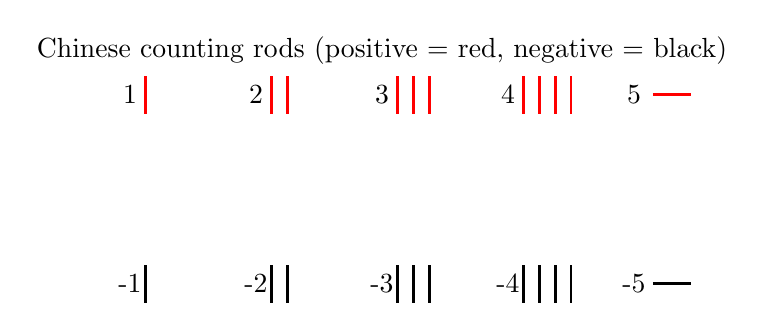
\begin{tikzpicture}[scale=0.8, line width=1pt]
		\node at (4,3.2) {Chinese counting rods (positive = red, negative = black)};
		% Positive numbers (red)
		\foreach \n/\count in {1/1, 2/2, 3/3, 4/4} {
			\node at (2*\n-2,2.5) {\n};
			\foreach \i in {1,...,\count} {
				\draw[red] (2*\n-2+0.25*\i,2.2) -- (2*\n-2+0.25*\i,2.8);
			}
		}
		\node at (8,2.5) {5};
		\draw[red] (8.3,2.5) -- (8.9,2.5);
		% Negative numbers (black)
		\foreach \n/\count in {1/1, 2/2, 3/3, 4/4} {
			\node at (2*\n-2,-0.5) {-\n};
			\foreach \i in {1,...,\count} {
				\draw[black] (2*\n-2+0.25*\i,-0.8) -- (2*\n-2+0.25*\i,-0.2);
			}
		}
		\node at (8,-0.5) {-5};
		\draw[black] (8.3,-0.5) -- (8.9,-0.5);
	\end{tikzpicture}
	\caption{Chinese counting rods: positive numbers (red), negative numbers (black).}
	\label{fig:rod_numerals_colored}
\end{figure}

\begin{MathBox}[Calculation Rules for Negative Numbers]
	\phantomsection\label{box:negative}
	Today the rules are familiar:
	\[
	(+a)+(-b)=a-b, \quad (-a)+(-b)=-(a+b),
	\]
	\[
	(-a)\cdot(-b)=+ab, \quad (-a)\cdot b=-(ab).
	\]
	Yet these simple rules were accepted only late in Europe.
	\textbf{René Descartes}\index{Descartes, René}
	still referred to negative numbers as ``false numbers.''
\end{MathBox}

The difficulty was obvious:
how could one possess something
that is less than nothing?
A negative result seemed absurd to many.
Only through applications such as bookkeeping,
temperature measurement, and later coordinate geometry
did their meaning become increasingly understandable.

With zero and the negative numbers,
the number system therefore expanded fundamentally.
Mathematics no longer described only the counting of existing things,
but also absence, losses, opposites, and directions.
Thus the modern number line emerged,
on which all integers from $-\infty$ to $+\infty$
can be arranged as an ordered structure.

This step, too, shows once again:
new kinds of numbers are not invented arbitrarily.
They become necessary
where the description of reality with the previous numbers reaches its limits.

\newpage
\noindent

% =====================================================
% 2.4 Complex Numbers -- an Unexpected Extension
% =====================================================
\subsection{Complex Numbers -- an Unexpected Extension}
\label{sec:2.4_complex}

\subsubsection*{Introduction}
\phantomsection
While fractions, irrational numbers, zero, and negative numbers each emerged
from practical or conceptual problems,
the next extension of the concept of number initially arose
as a by-product of algebraic solution methods:
the so-called \emph{complex numbers}.
They appeared when equations were investigated
that could not be solved completely with the number types known up to that point.

\subsubsection*{First Approaches in the Renaissance}
\phantomsection
In the sixteenth century, Italian mathematicians such as
\textbf{Scipione del Ferro}\index{del Ferro, Scipione},
\textbf{Niccolò Tartaglia}\index{Tartaglia, Niccolò}, and
\textbf{Gerolamo Cardano}\index{Cardano, Gerolamo}
worked on the solution of cubic equations.
In some solution procedures, intermediate steps involving $\sqrt{-1}$ appeared --
even though the final result was again a real number.
Cardano spoke in this context of ``sophistic roots.''
He did write down such expressions,
but their meaning remained unclear.
They appeared like a strange computational aid:
formally necessary, but without any intuitive place
in the known number system.

\subsubsection*{Bombelli and the Turning Point}
\phantomsection
The Italian mathematician \textbf{Rafael (Raffaele) Bombelli}\index{Bombelli, Rafael}
recognized around 1572
that one can calculate consistently with these ``imaginary numbers''
if clear rules of calculation are introduced and, in particular, one sets $i^2=-1$.
With this, he laid the foundation
for the later theory of complex numbers.

For a long time, complex numbers were still regarded as ``fictitious'' or ``imaginary.''
Only in the eighteenth and nineteenth centuries,
especially through the work of \textbf{Leonhard Euler}\index{Euler, Leonhard},
\textbf{Carl Friedrich Gauss}\index{Gauss, Carl Friedrich}, and
\textbf{Jean-Robert Argand}\index{Argand, Jean-Robert},
did the insight prevail:
complex numbers are not merely formal aids,
but a necessary and fully valid extension of the concept of number.

\subsubsection*{Significance}
\phantomsection
Today the complex numbers form a foundation of modern mathematics.
In the \emph{fundamental theorem of algebra}\index{fundamental theorem of algebra},
they ensure that every nonconstant polynomial over the complex numbers
has at least one root.
This makes clear
that the complex numbers are not merely an artificial addition,
but represent a completion of the algebraic concept of number.

They are also indispensable in physics and engineering --
for example in oscillations, waves,
in quantum mechanics,
and in electrical engineering.
What initially appeared to be a formal peculiarity
thus turns out to be a deep structure of modern science.

The detailed historical derivation
and the formal introduction of $i^2=-1$
can be found in Appendix~\ref{anhangA_komplexe}.

% =====================================================
% 2.5 Conclusion
% =====================================================

\subsection{Conclusion: Numbers as Discovered Structure}

From counting herds to the introduction of complex numbers,
a continuous thread becomes visible:
new kinds of numbers do not arise arbitrarily,
but whenever the previous numbers are no longer sufficient
to describe mathematical or real relationships.

\begin{itemize}
	\item The \emph{natural numbers}\index{natural numbers}
	arose from the practical need to distinguish and count quantities.
	\item \emph{Irrational numbers}\index{irrational numbers}
	became necessary when geometry produced quantities
	that could no longer be expressed by fractions.
	\item \emph{Zero}\index{zero}
	and the \emph{negative numbers}\index{negative numbers}
	expanded the concept of number to absence, losses, opposites, and directions.
	\item The \emph{complex numbers}\index{complex numbers}
	opened up a domain in which algebraic problems
	become generally solvable and which is fundamental
	to modern mathematics and physics.
\end{itemize}

\begin{NoteBox}[Numbers as Universal Structure]
	\phantomsection\label{box:universal_numbers}
	Numbers are not merely free inventions of human beings.
	Their signs, names, and forms of representation did arise culturally,
	but the structures to which they refer are not arbitrary.
	They are discovered step by step,
	because reality and the inner logic of mathematics
	force ever new domains of number --
	from the first notches on bones
	to the complex plane.
\end{NoteBox}